\section{Databases}
Some databases has been used in order to learn, compare results and carry out the project. All the databases are formed by three subsets whose samples are not repeated among subsets: train, validation and test.

\begin{itemize}
\item The training subset is used to train the network during epochs. To know how the training behavior, a cost is calculated.
\item The validation subset is used to check the behavior of the network while is training, also, the validation subset is usually used to calculate the hyper-parameters of the network, although the hyper-parameters are not calculated until is pointed. The validation error is calculated for each training epoch. The metric use to the validation is $error(\%) = cost*100$.
\item  The test subset, that is used just at the end of the training. The best model is chosen with regard to the best validation error. Different metrics are going to be used for after testing the network (error (\%), TP, FP ...).
\end{itemize}

\subsection{MNIST digit database}\label{subsec:MNIST}
MNIST digit database is a image database of human written digits. This database is commonly used to learn machine learning techniques. Because of that, this database has been used in order to learn Theano and convolutional neural networks. In addition, this database has been used in a implemented convolutional neural network (LeNet).\\
\begin{figure}[htb]
\centering
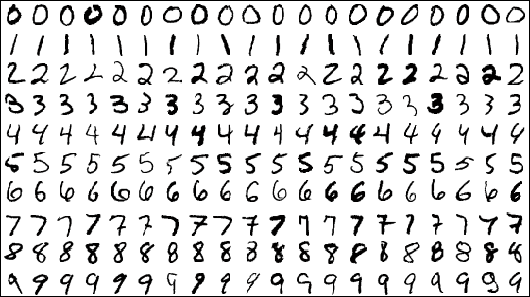
\includegraphics[width=0.7\textwidth]{images_databases/mnistExamples.png}
\caption{digits MNIST images database} \label{fig:MNIST_digits}
\end{figure}
Some examples of the digit image MNIST database could be seen in \ref{fig:MNIST_digits} and the characteristics of this database are the following ones:

\begin{itemize}
 \item Number of samples: 70.000 number of unique samples.
 \item Number of features/ length of each image: 784
 \item Number of classes: 10, one per digit
\item The size of each image is 28x28 pixels.
\item The images are in grey scale.
\end{itemize}

\subsection{Labeled faces in the wild}
\textit{The Labeled Faces in the Wild} is a well-known and used dataset of faces images that can be found in its official web page \url{http://vis-www.cs.umass.edu/lfw/}.\\

The characteristics of this database are the following ones:
\begin{itemize}
 \item Number of samples/ Number of images : 13233
 \item Number of features/ length of each vectorized image: 187500
 \item Number of classes / Number of people: 5748
\item The number of images per person is not the same for each one.
\item The size of each image is 250x250 pixels.
\item The images are RGB ones.
\item The faces in images are in the center of the image.\\
\end{itemize}
\begin{figure}[htb]
\centering
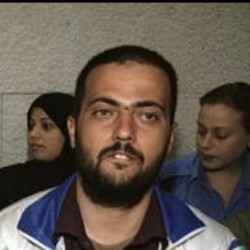
\includegraphics[width=0.2\textwidth]{images_databases/LFW/1.jpg}
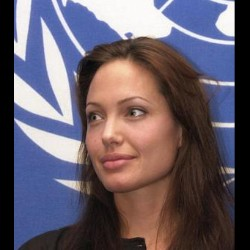
\includegraphics[width=0.2\textwidth]{images_databases/LFW/2.jpg}
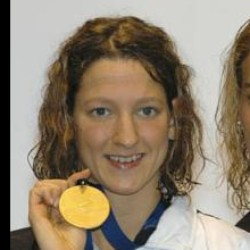
\includegraphics[width=0.2\textwidth]{images_databases/LFW/3.jpg}
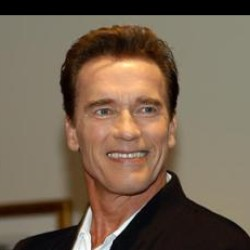
\includegraphics[width=0.2\textwidth]{images_databases/LFW/4.jpg}
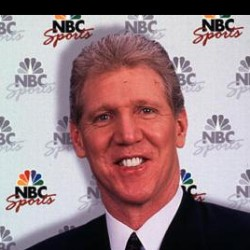
\includegraphics[width=0.2\textwidth]{images_databases/LFW/5.jpg}
\caption{Examples of Labeled faces in the wild imamges} \label{fig:LFW1}
\end{figure}

Examples of images of this database could be seen in figure \ref{fig:LFW1} in which faces of well-known people are visualized.\\


This database has been used to learn; to learn how to read a database, how to feed the network with those images.\\

\subsection{FRAV dataset}
FRAV database is an anti-spoofing face database built in the research group of tu URJC called FRAV. This dataset is formed by five different classes:\\

\begin{itemize}
 \item Original images of people.
 \item Images of people printed (attack).
 \item Images of people with a mask (attack).
 \item Images of pleople with a mask with the eyes cropped (attack).
 \item Images of people in a tablet (attack).\\
 \end{itemize}

There are the same number of samples in each class. The images of that classes can be found in RGB and NIR (not all RGB images has its corresponding NIR image). Characteristics of FRAV images ere the following ones:\\

\begin{itemize}
 \item There are 939 people in each RGB class or 195 in NIR class.
\item There is one image per person.
\item Each image h as it is own shape.
\item The faces in images are in the center of the image.\\
\end{itemize}

This images has been used in different ways, in some experiments, just RGB images has been used, so 939 images has been used. When has been used RGB and NIR images at the same time, 195 images has been used (195 RGB and its corresponding NIR). To classify, two different ways has been used; the first one where real people formed one class and the different attacks formed other class, so two classes have been used; and the second way where each attacks correspond with a class, so five classes (4 attacks and 1 real) have been used.\\

One exaple of RGB images of FRAV database are shown in figure \ref{fig:RGB-frav1} and another example could be seen in \ref{fig:RGB-frav2}. In both images, the four attacks described previously and the real user could be visualized. \\

\begin{figure}[htb]
\centering
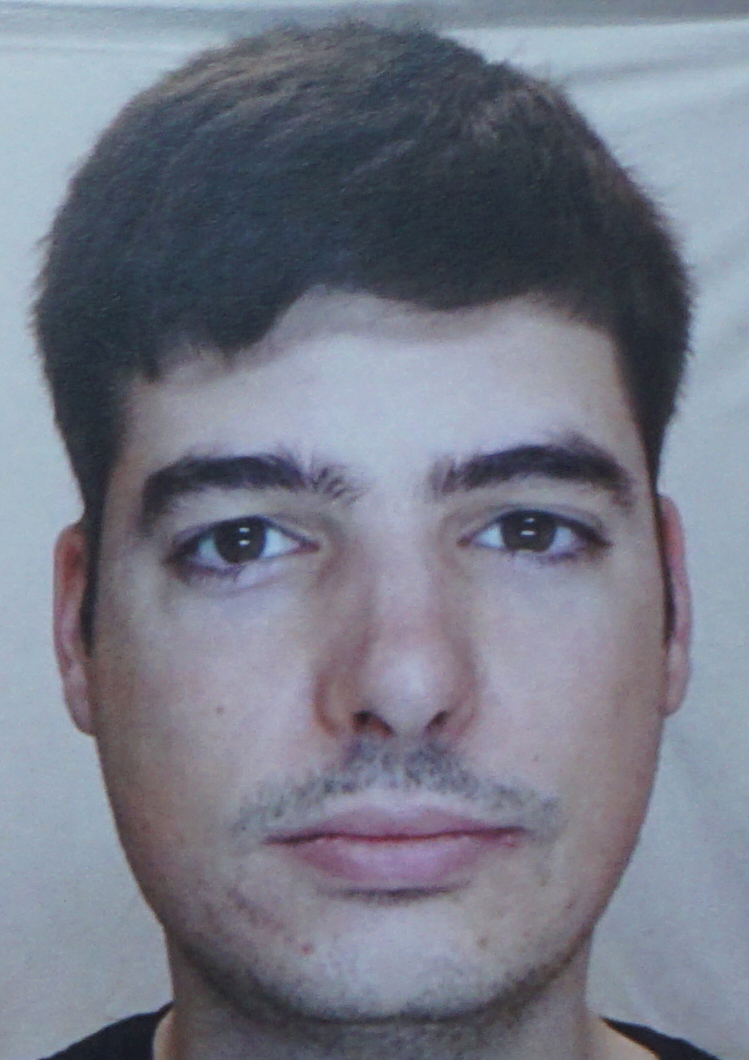
\includegraphics[width=0.18\textwidth]{images_databases/fravrgb/at1-0.JPG}
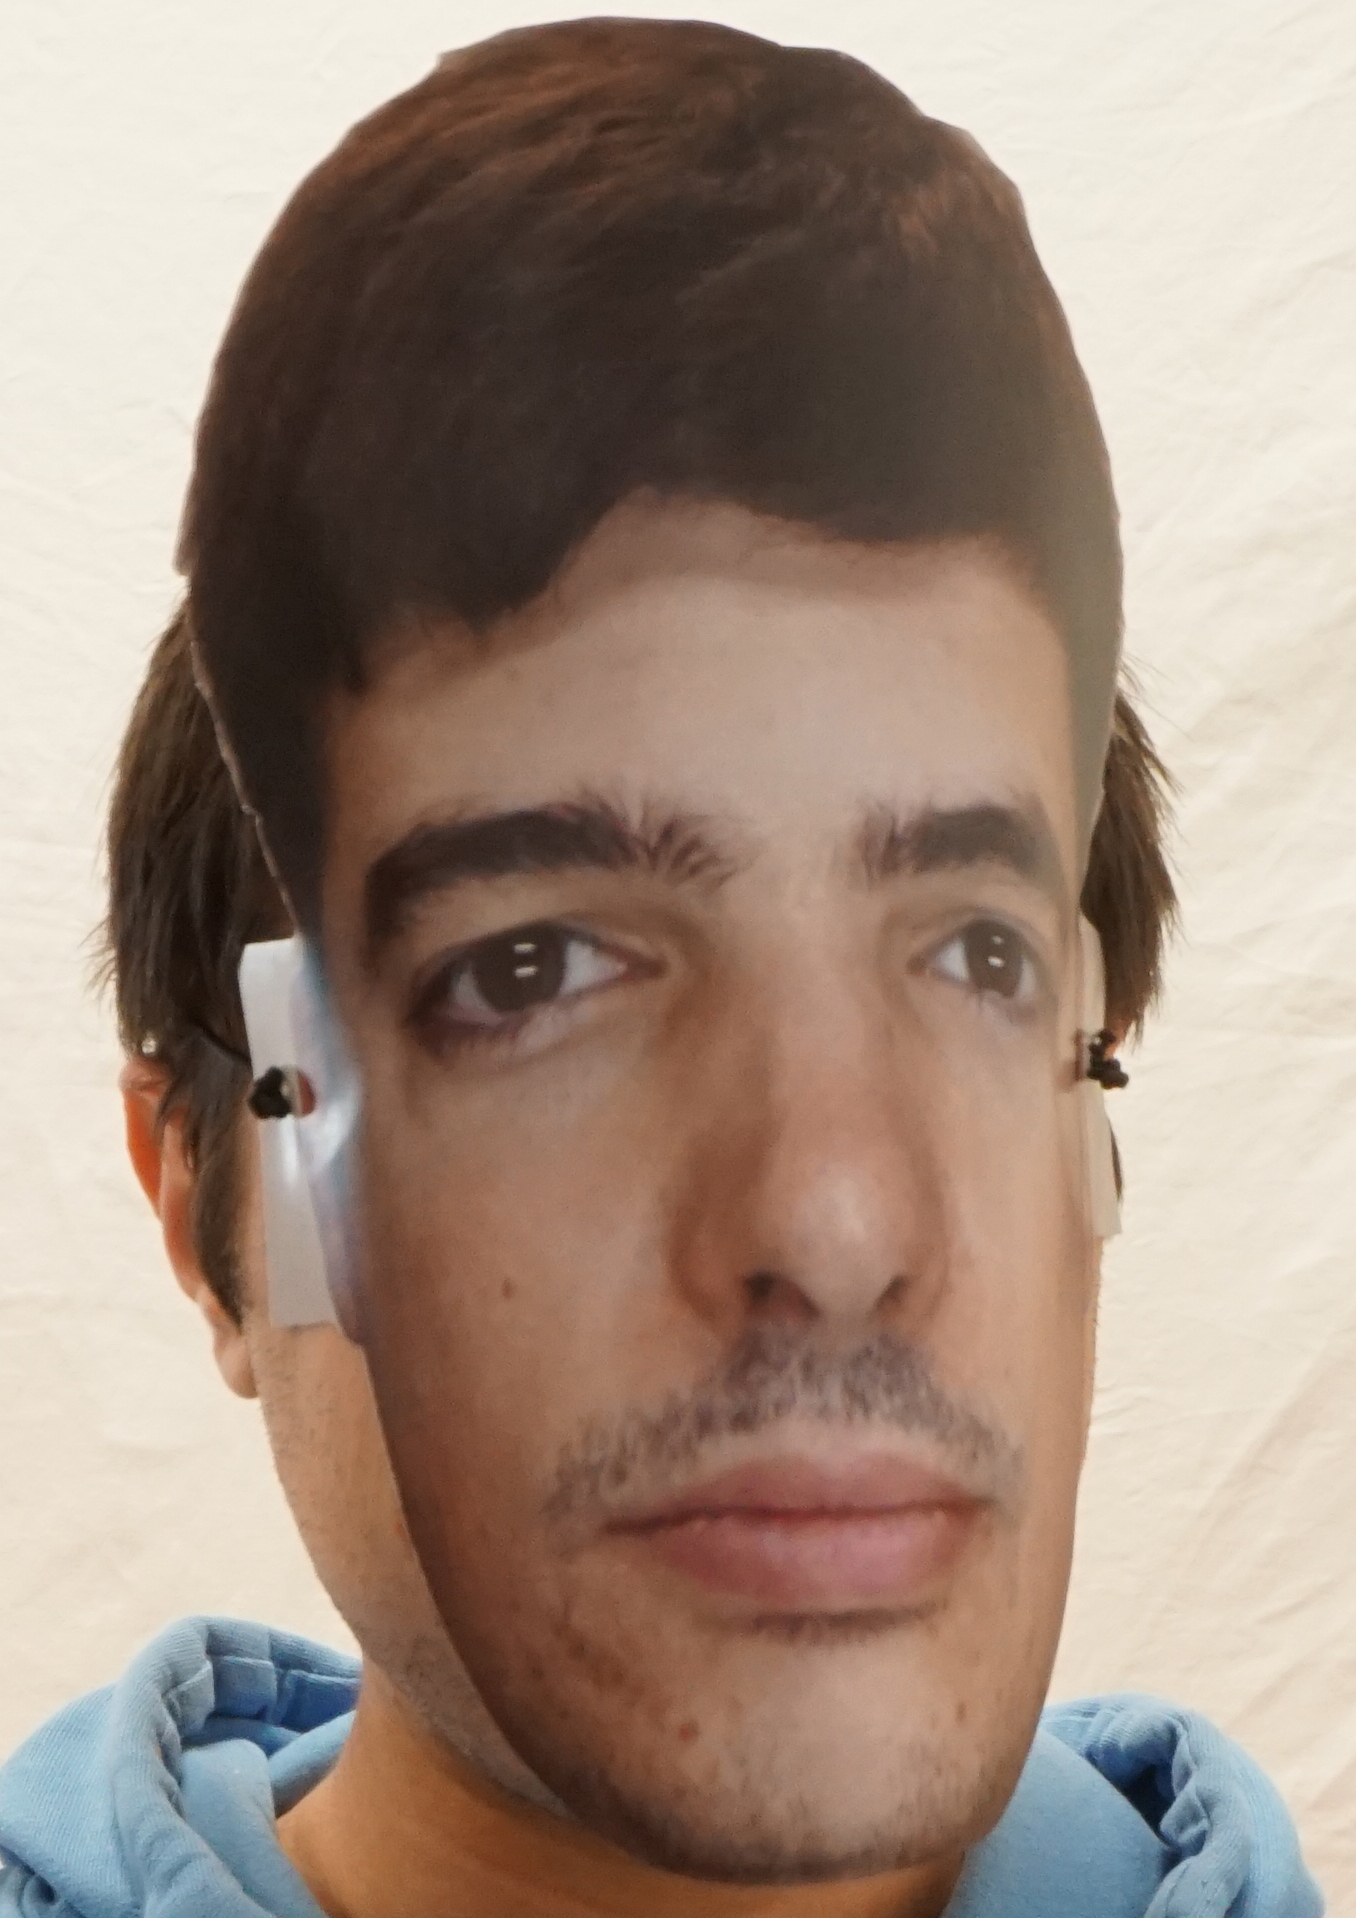
\includegraphics[width=0.18\textwidth]{images_databases/fravrgb/at2-0.JPG}
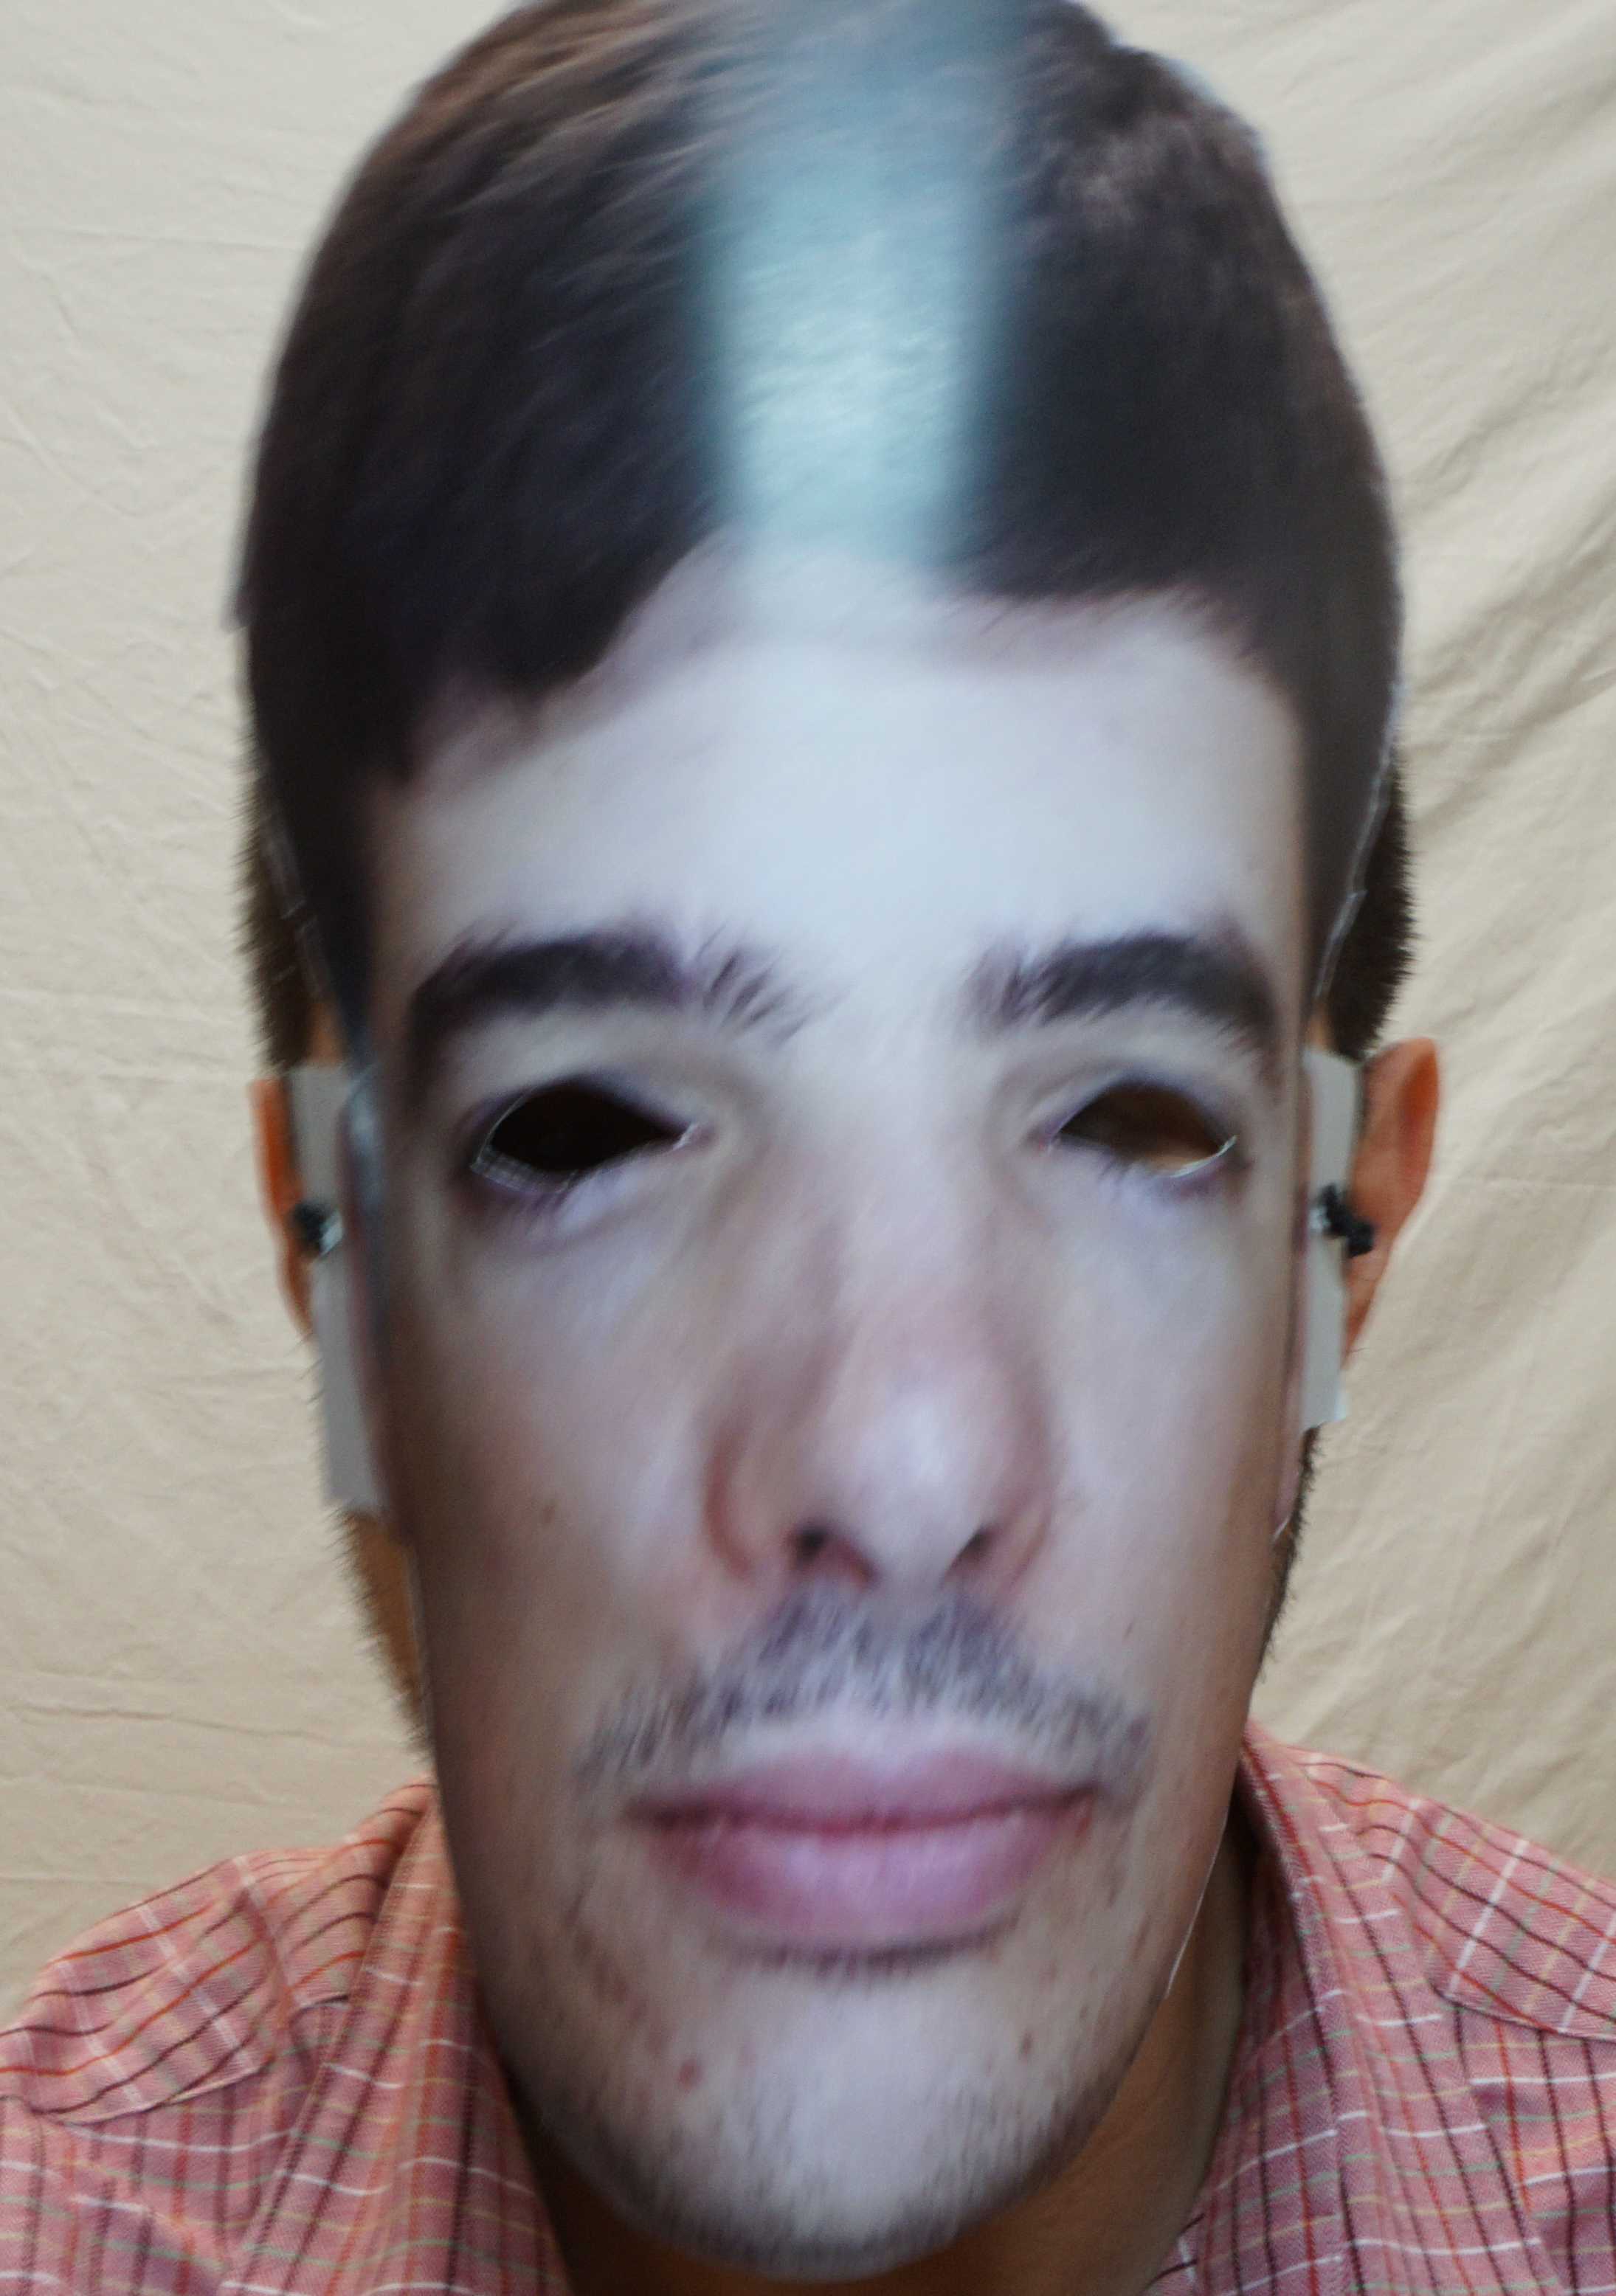
\includegraphics[width=0.18\textwidth]{images_databases/fravrgb/at3-0.JPG}
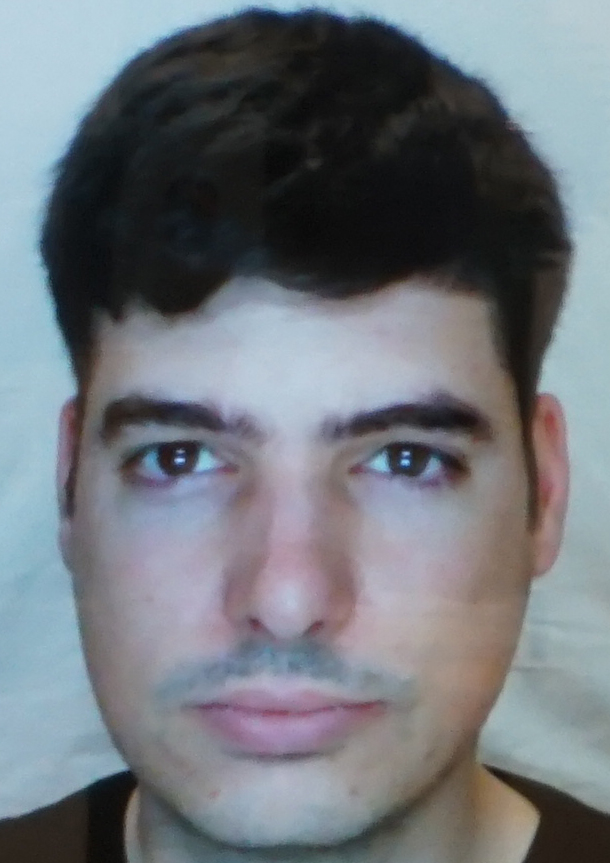
\includegraphics[width=0.18\textwidth]{images_databases/fravrgb/at4-0.JPG}
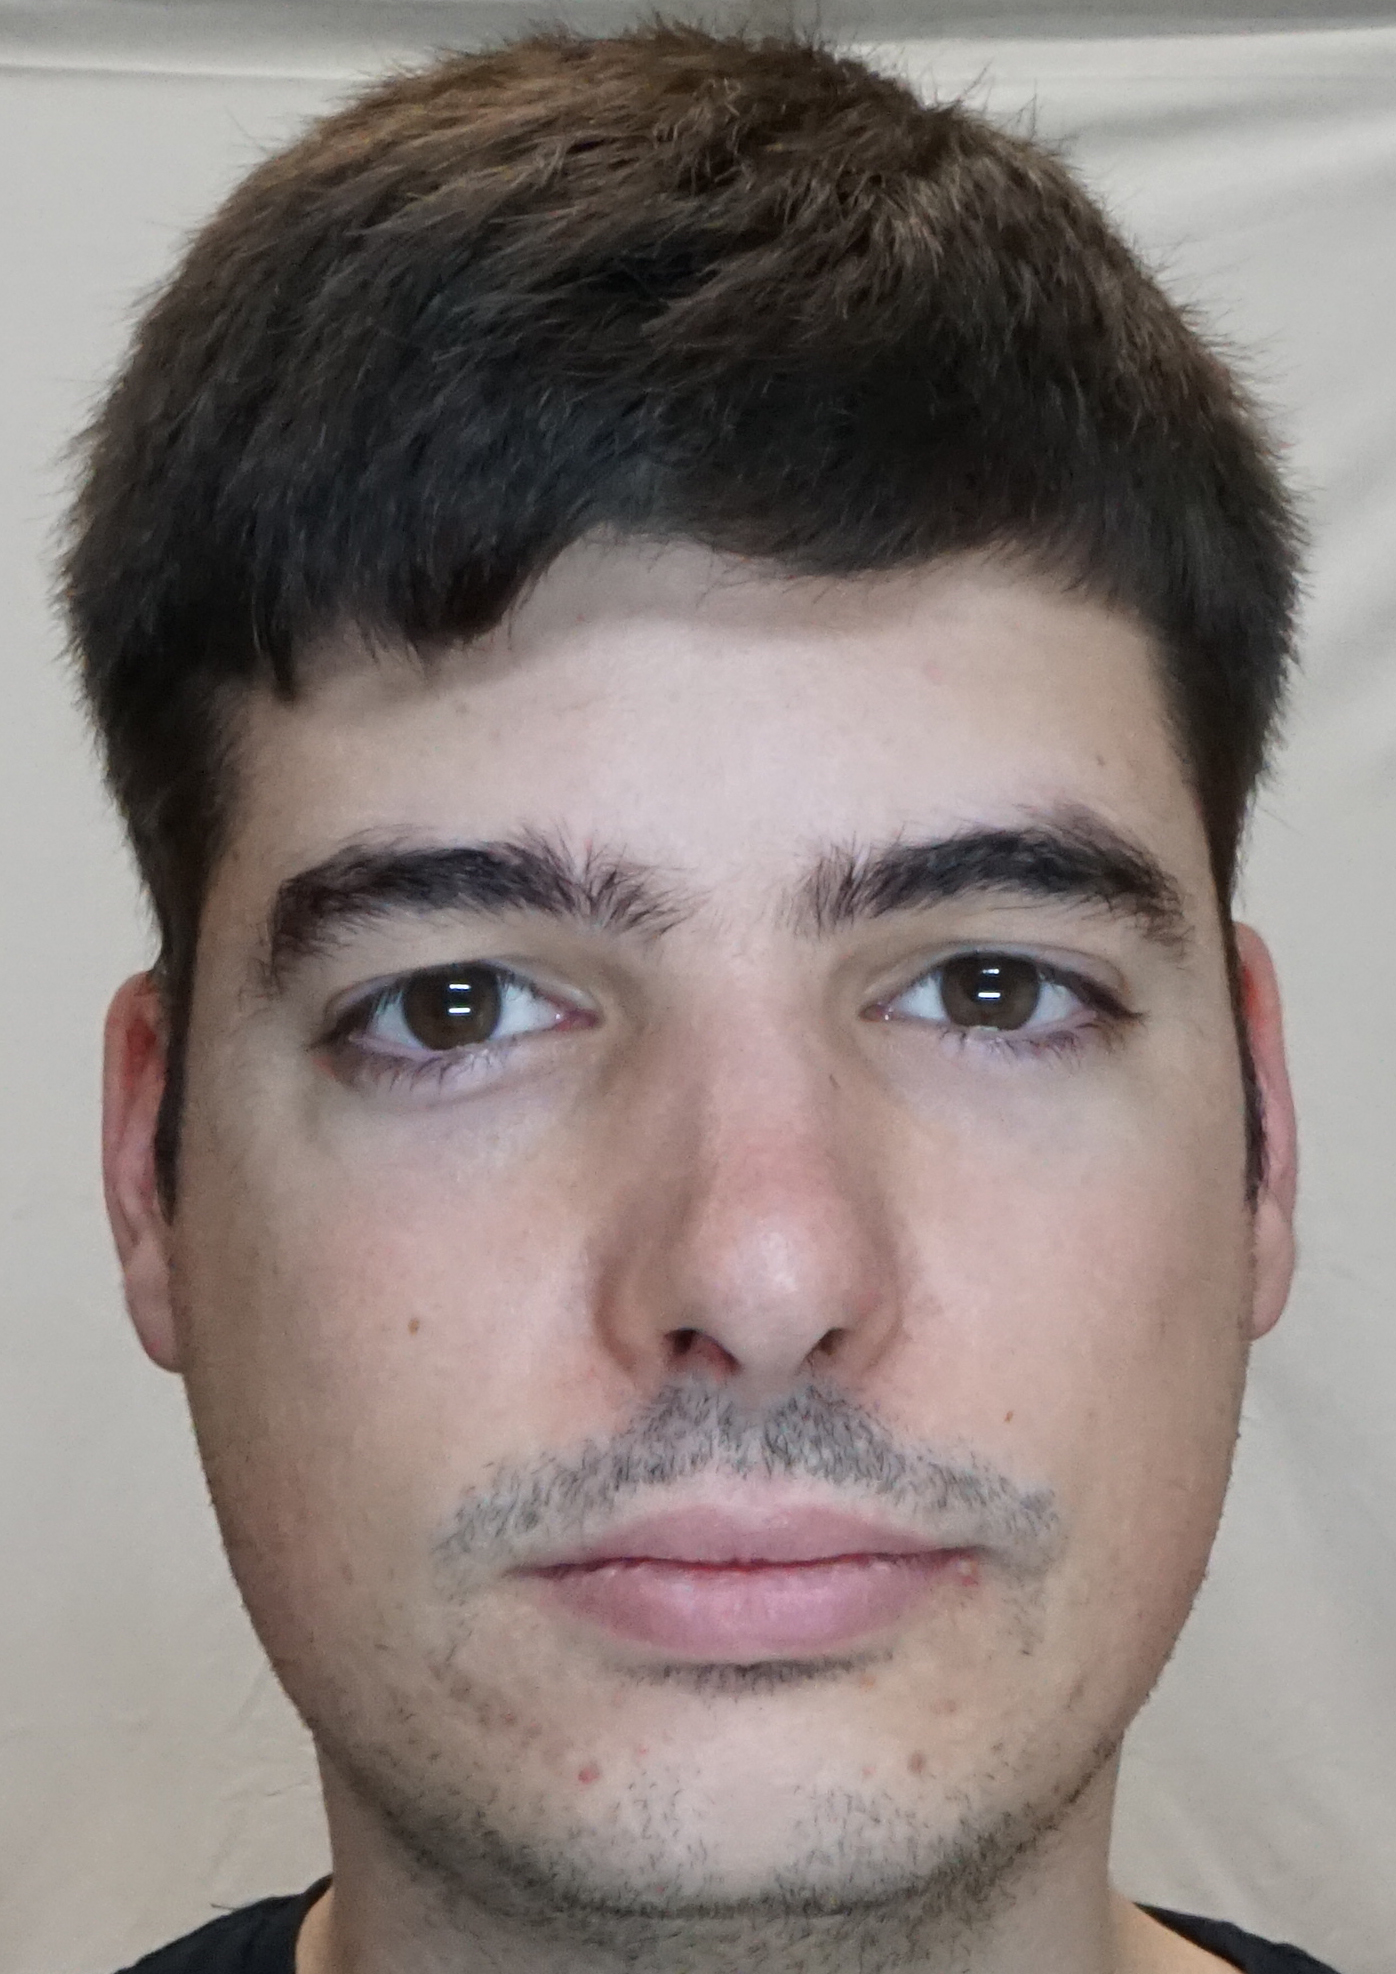
\includegraphics[width=0.18\textwidth]{images_databases/fravrgb/real0.JPG}

\caption{Four attacks and real user from RGB FRAV database } \label{fig:RGB-frav1}
\end{figure}

\begin{figure}[htb]
\centering
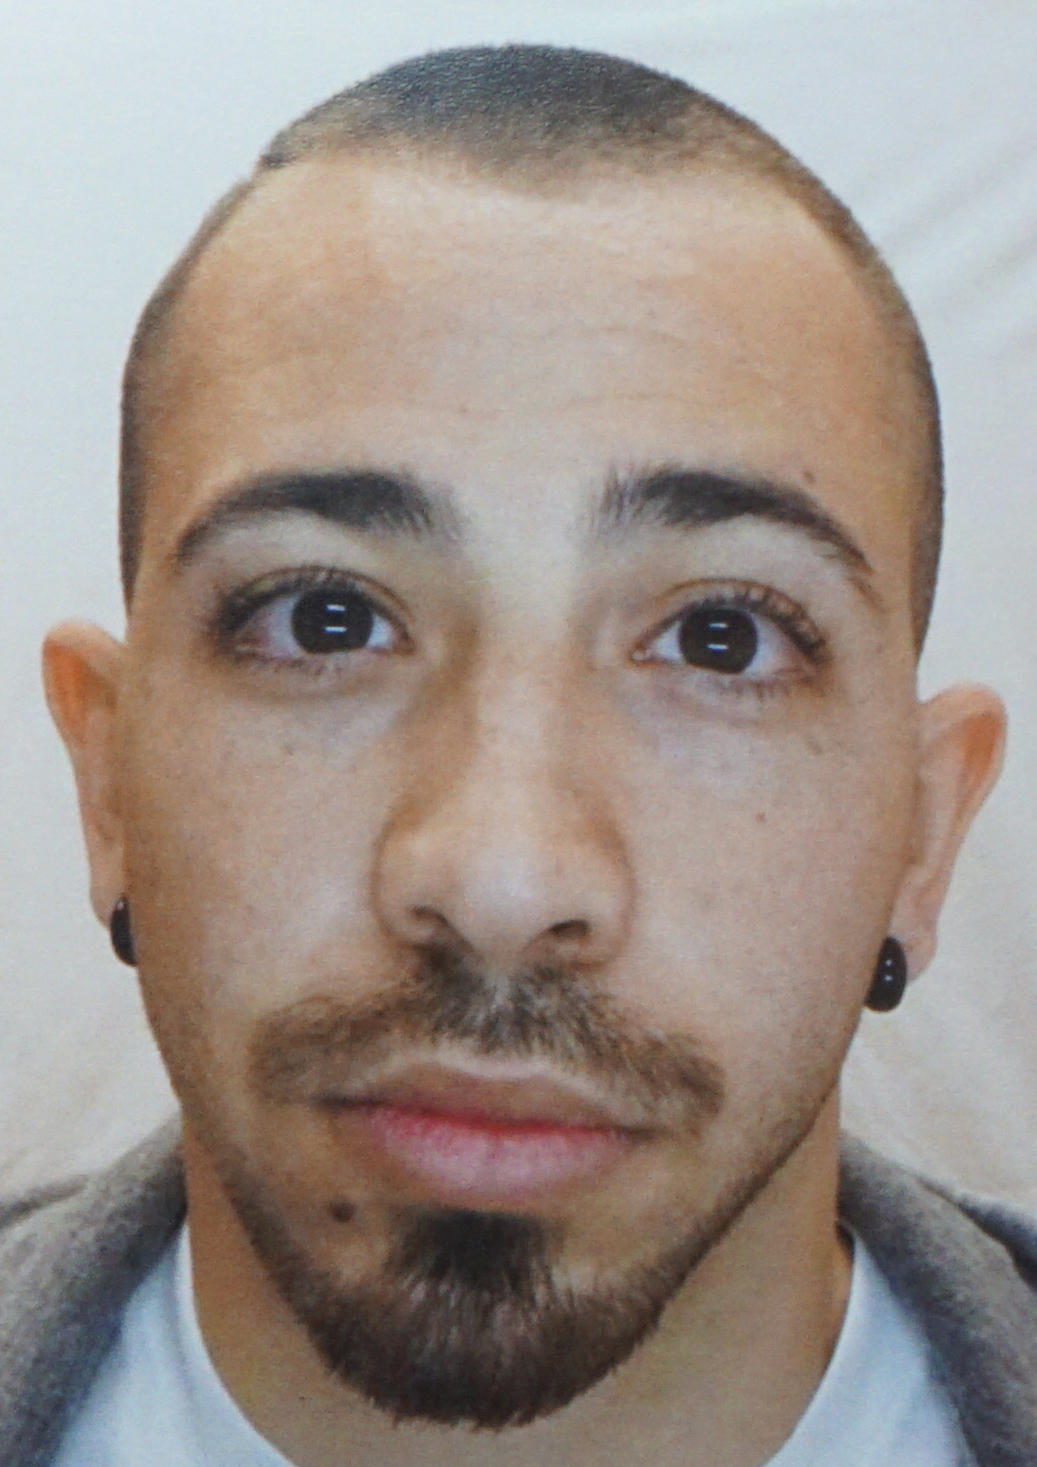
\includegraphics[width=0.18\textwidth]{images_databases/fravrgb/at1-1.JPG}
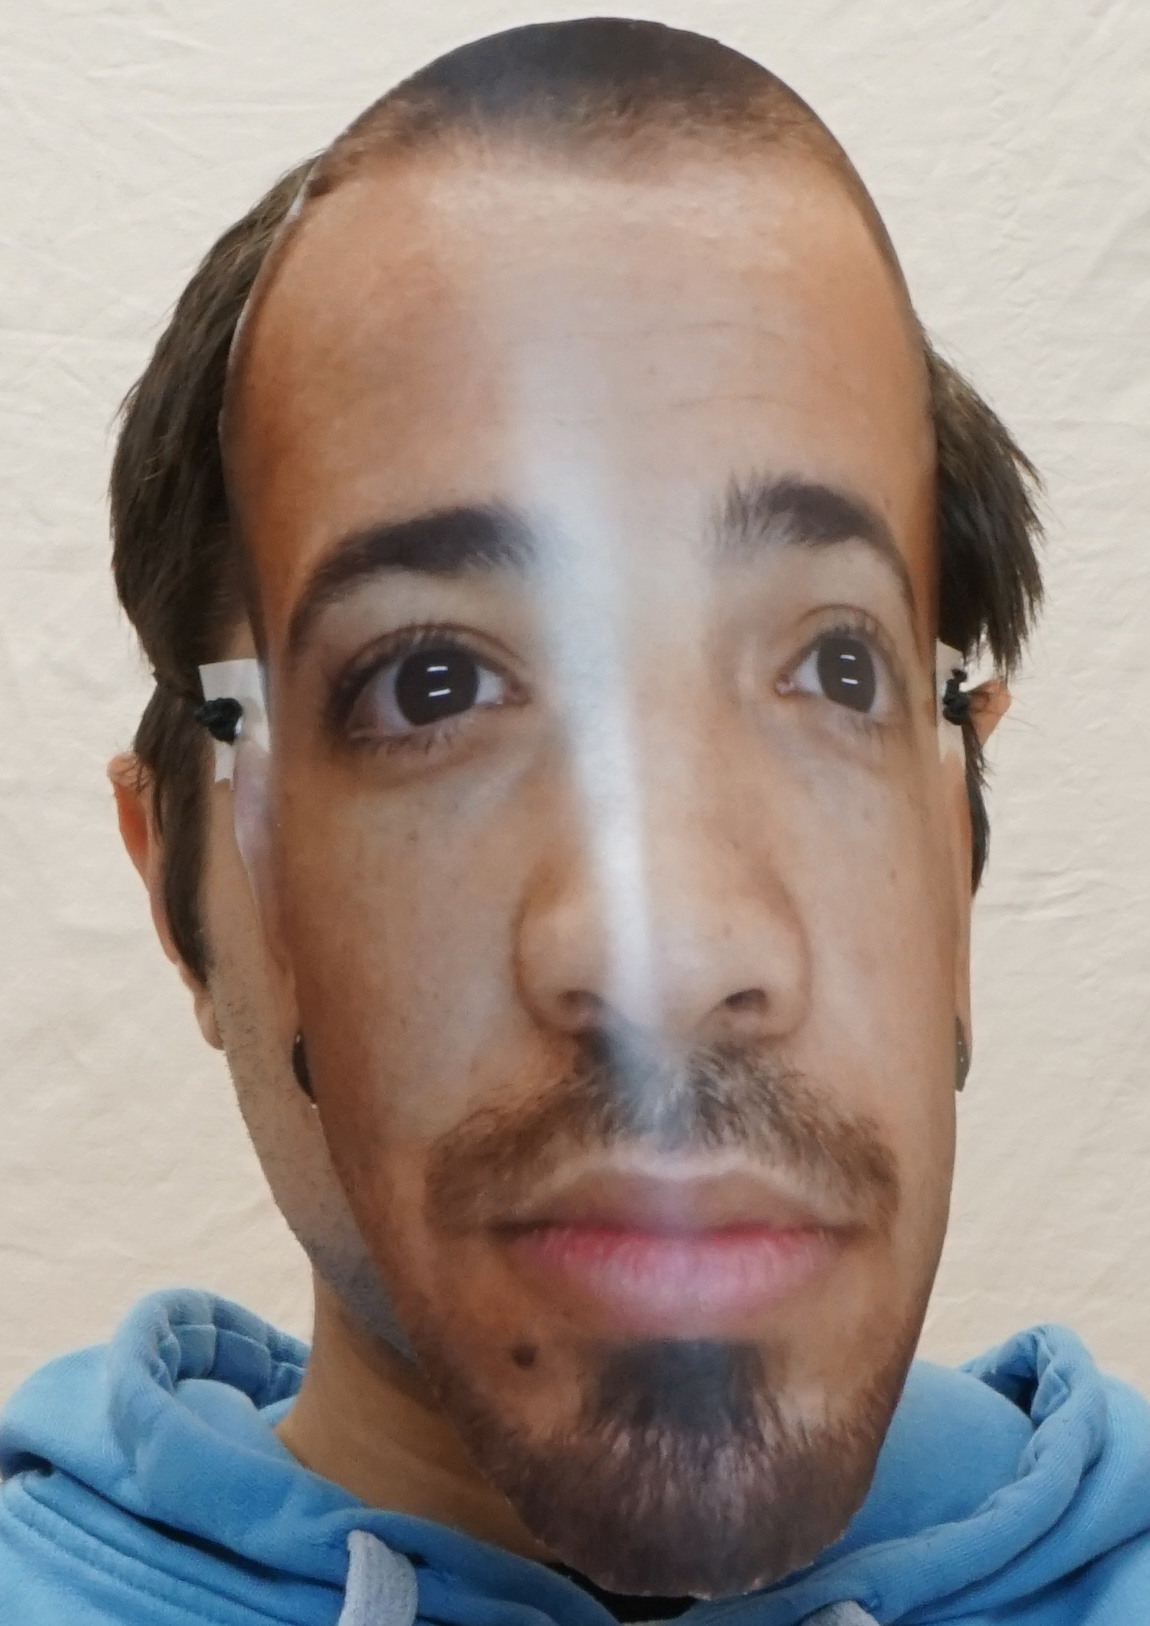
\includegraphics[width=0.18\textwidth]{images_databases/fravrgb/at2-1.JPG}
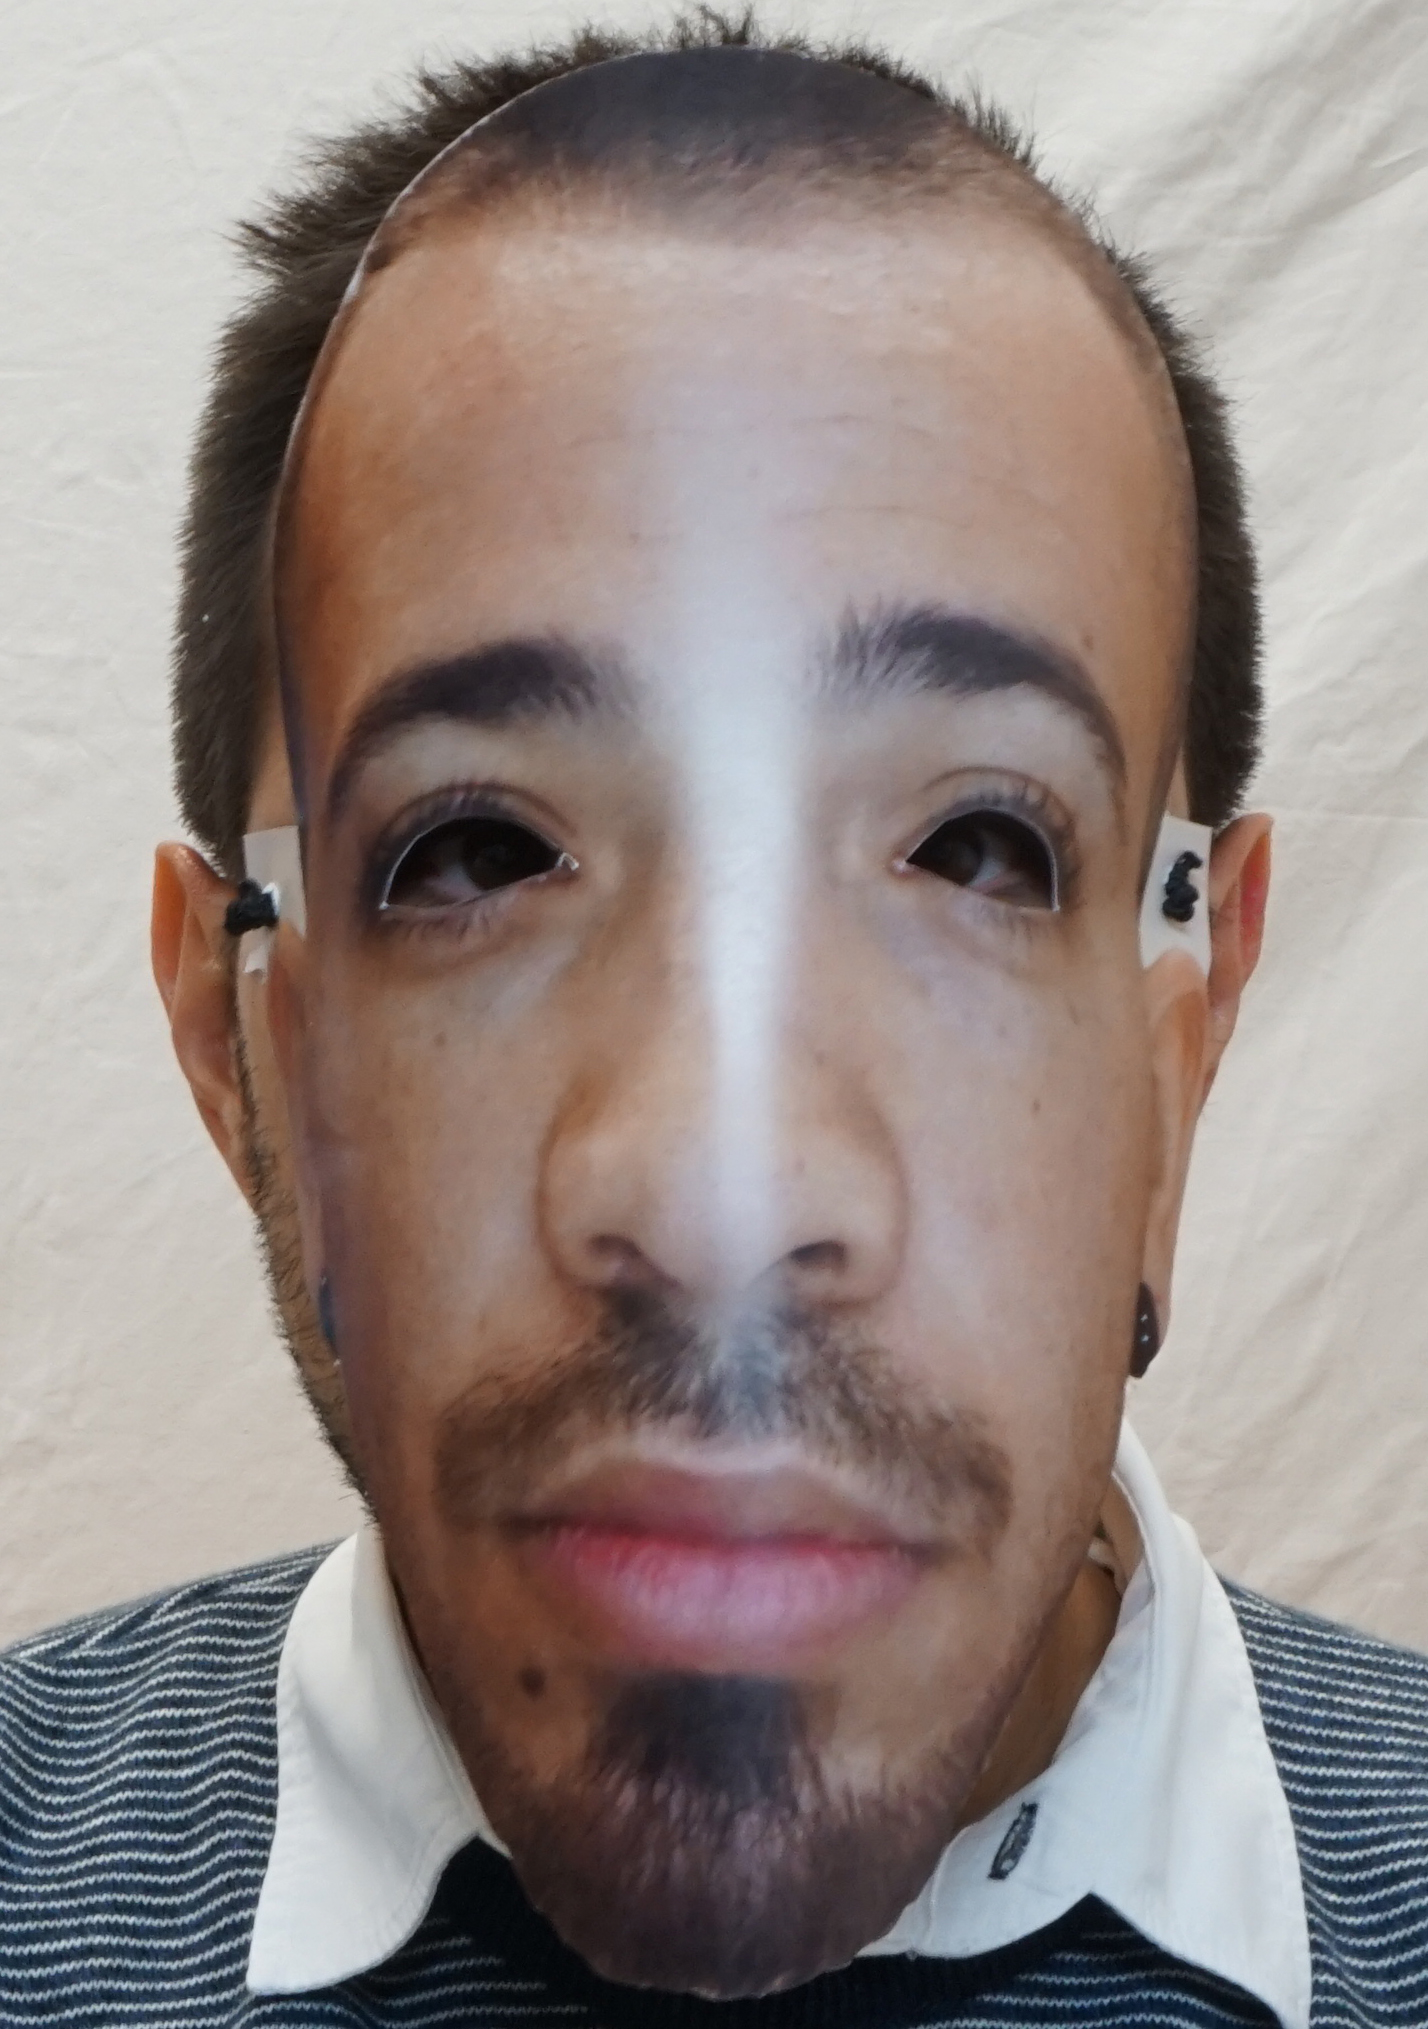
\includegraphics[width=0.18\textwidth]{images_databases/fravrgb/at3-1.JPG}
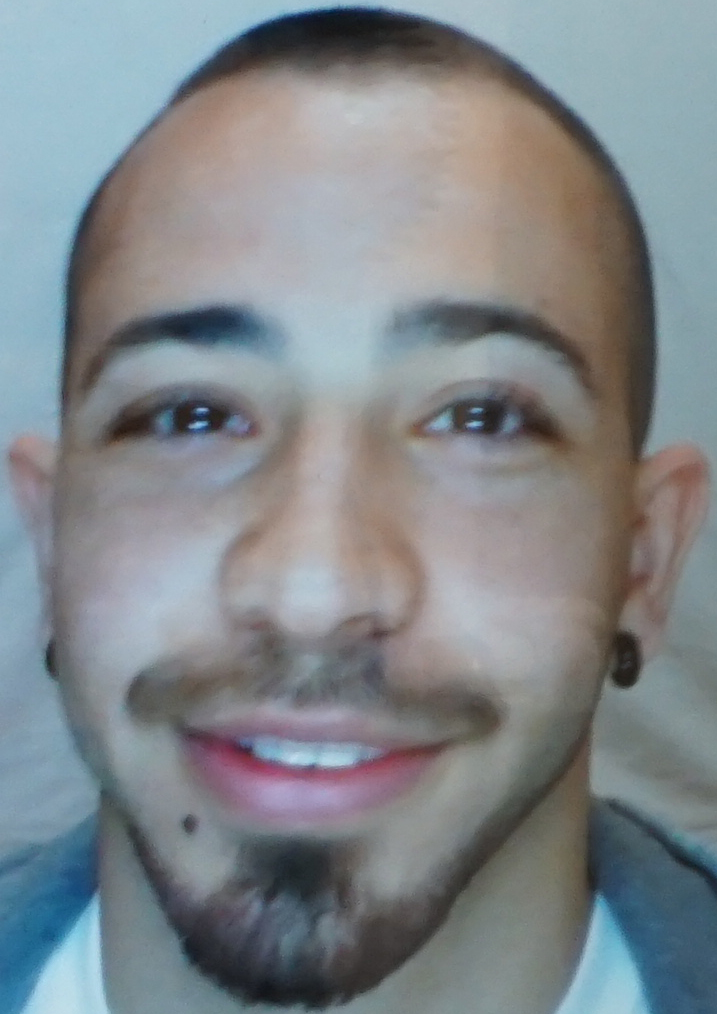
\includegraphics[width=0.18\textwidth]{images_databases/fravrgb/at4-1.JPG}
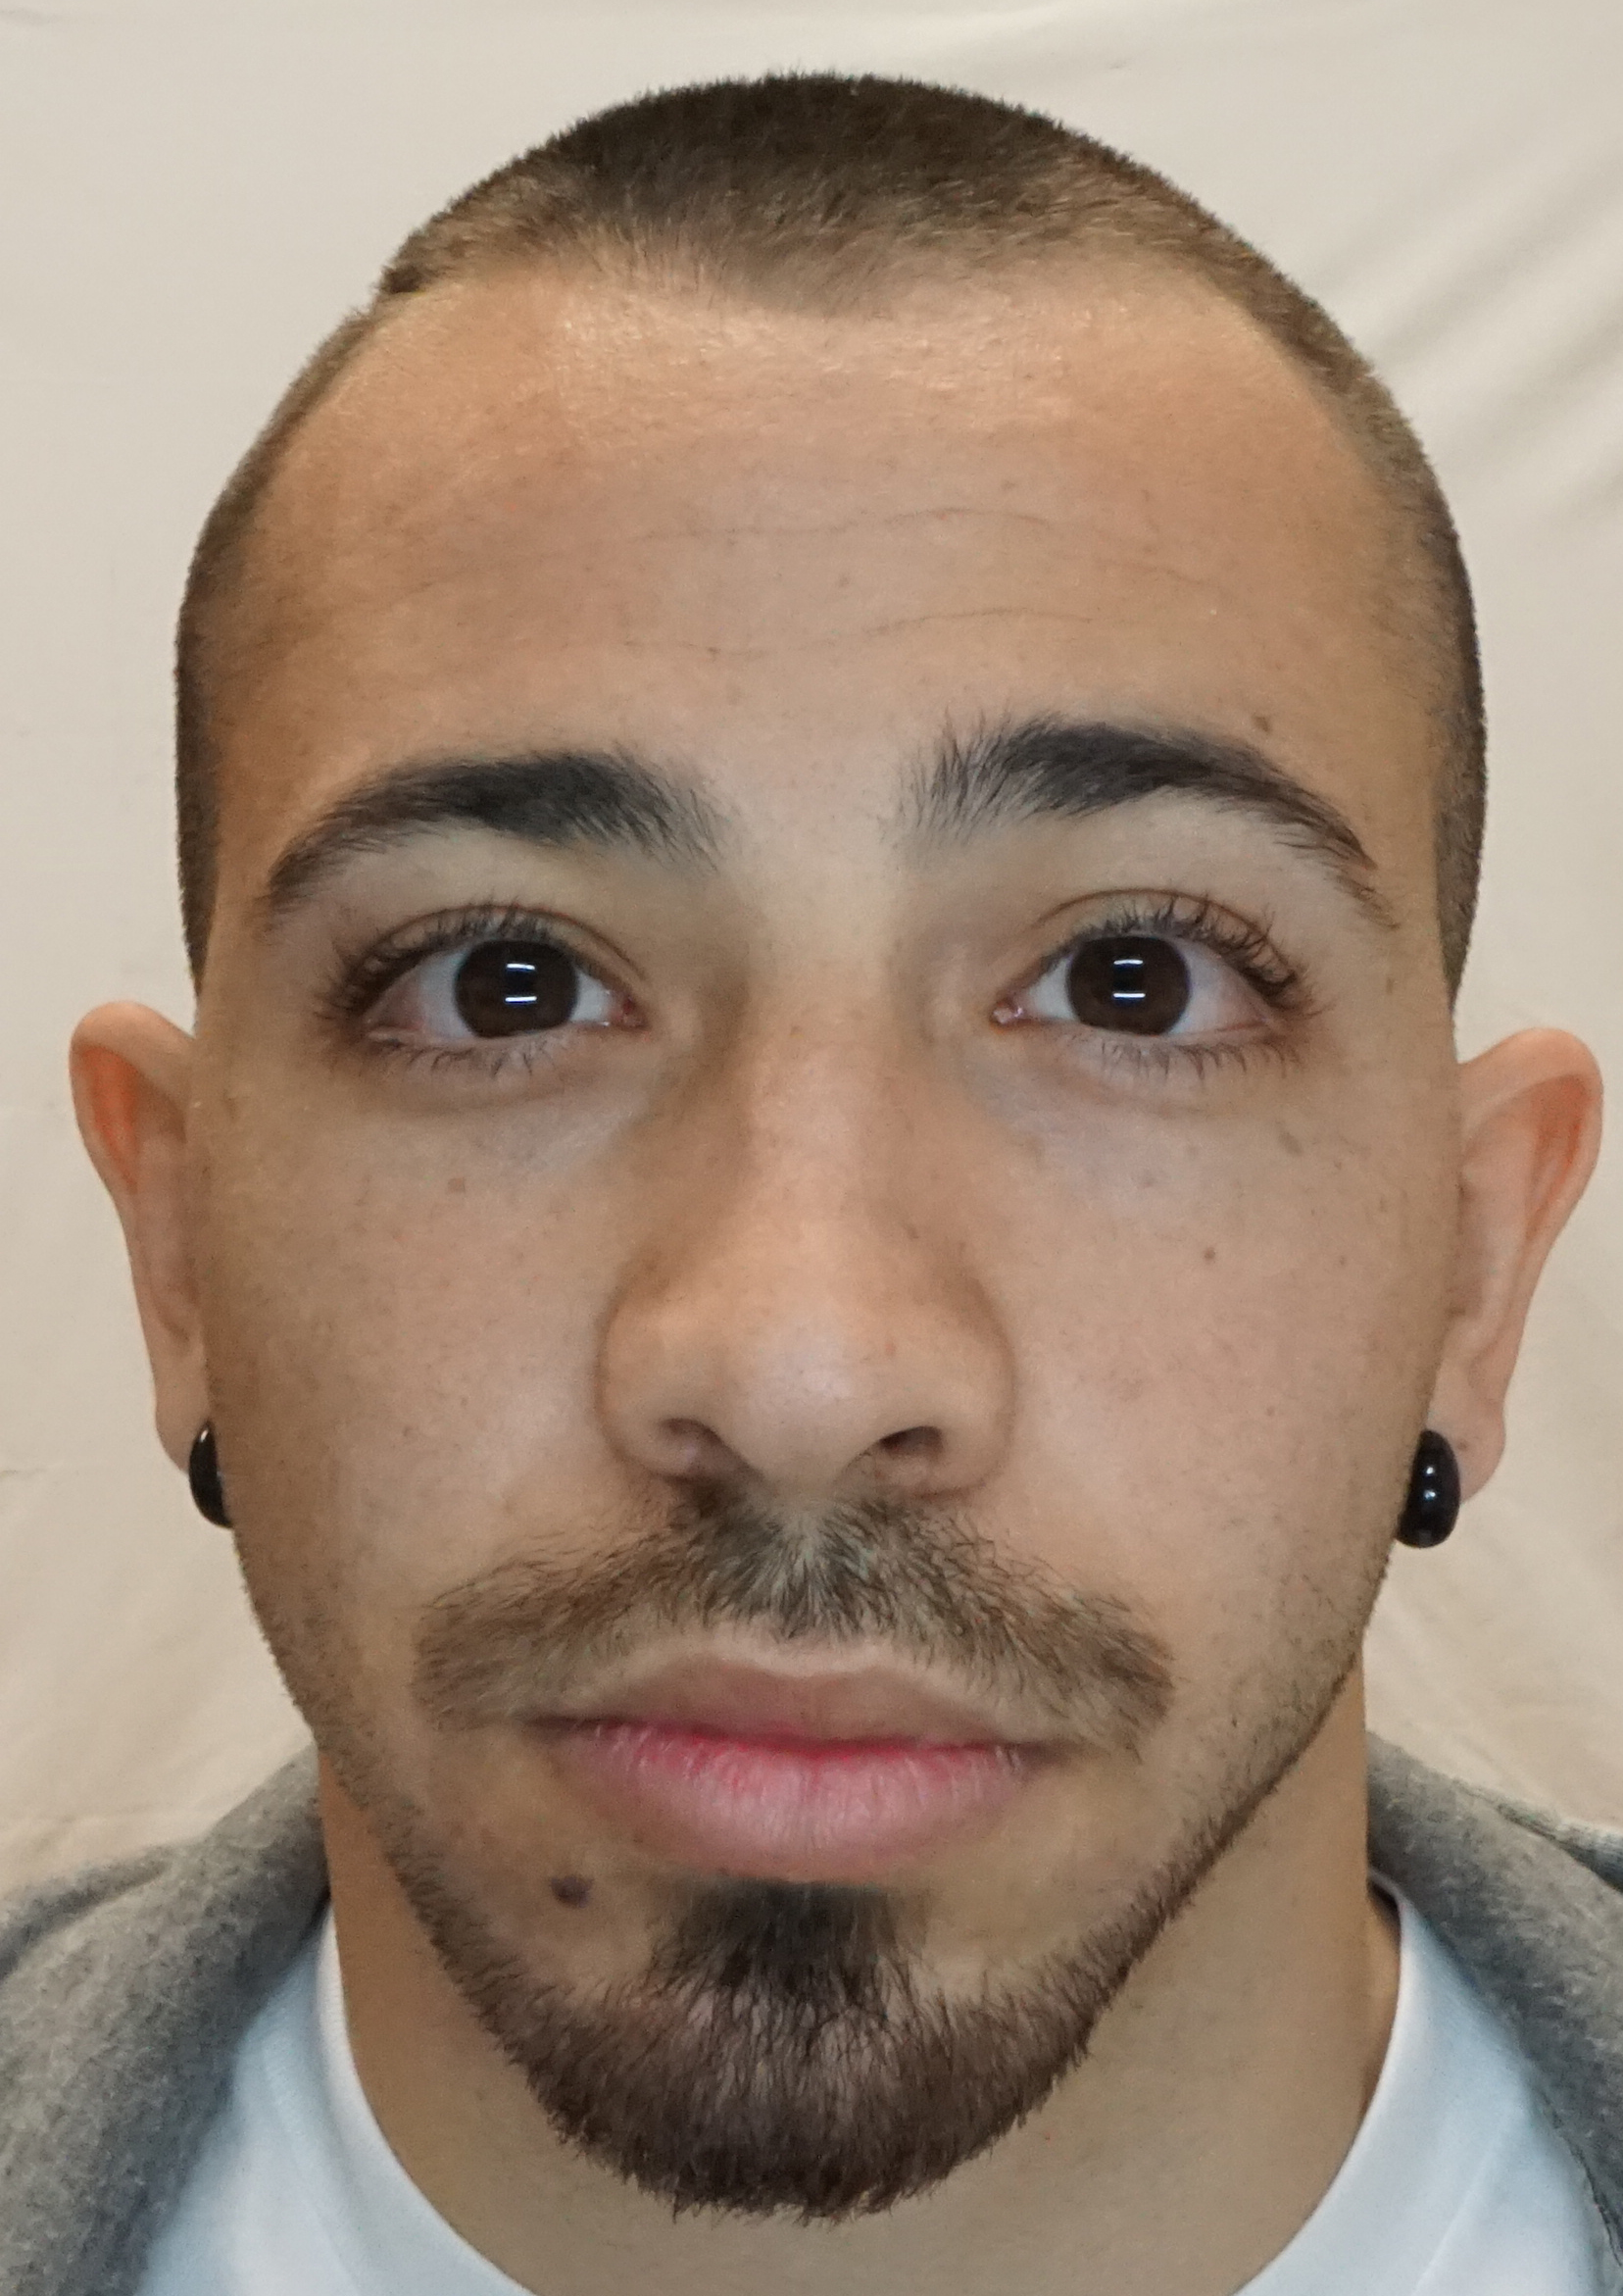
\includegraphics[width=0.18\textwidth]{images_databases/fravrgb/real1.JPG}

\caption{Four attacks and real user from RGB FRAV database } \label{fig:RGB-frav2}
\end{figure}

This database is used in different ways:
\begin{enumerate}
  \item Using the 933 people, in which each person would have a genuine image and four attacks.
  \item Using the 195 people which correspond with NIR images and its corresponding images in RGB.
\end{enumerate}

If RGB and NIR images are used at the same time, two different methods of using together are used:
\begin{itemize}
\item Characteristic level: adding the NIR image as another layer to RGB image, so the resultant image have hightxweightx4 dimensions (NIR images has one layer because it is a gray scale image and RGB images has tree layers, one per each primary color). The network is feed with the resultant images like other times.
\item Classification level: training two network twice, first, with RGB images and then with NIR images and when the classification is produced combine them.
\end{itemize}

\subsection{CASIA dataset}
Casia is a face anti-spoofing database built in the center for Biometrics and security research.\\

In the same way as FRAV dataset, this database is formed by real or genuine images of people and three different attacks of the same people:

\begin{itemize}
 \item Images of people printed (attack).
 \item Images of people with a mask (attack).
 \item Images of people with a mask with the eyes cropped (attack).
 \end{itemize}


\begin{itemize}
\item There are 939 people in each RGB class or 195 in NIR class.
\item There is one image per person.
\item The size of each image is 720x1280 pixels.
\item The faces in images are in the center of the image.\\
\item Images are RGB.
\end{itemize}


Two people of Casia database could be seen in figure \ref{fig:casia1} and figure \ref{fig:casia2}, where three attacks types could be seen with the real user of both examples.

\begin{figure}[htb]
\centering
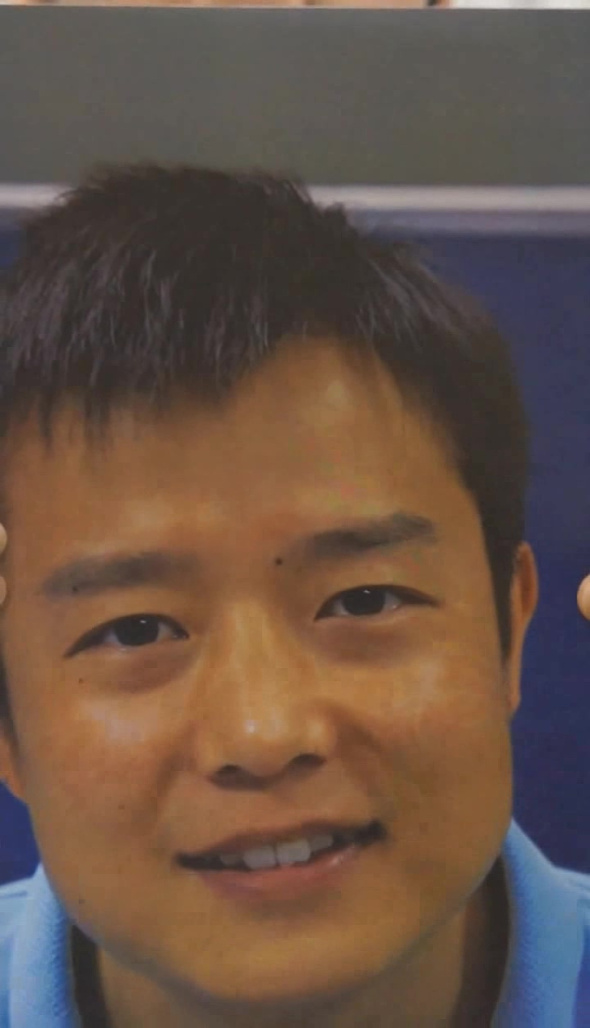
\includegraphics[width=0.2\textwidth]{images_databases/casia/at1-2.jpg}
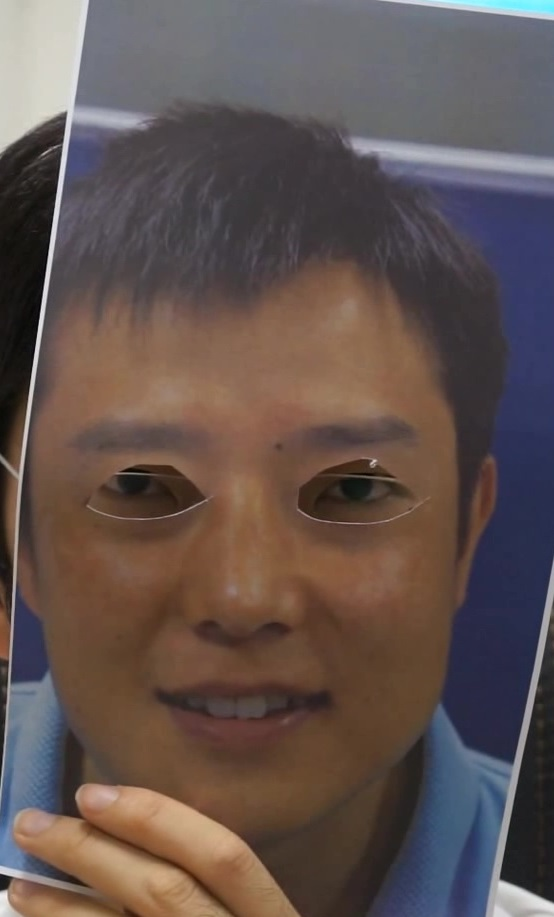
\includegraphics[width=0.2\textwidth]{images_databases/casia/at2-2.jpg}
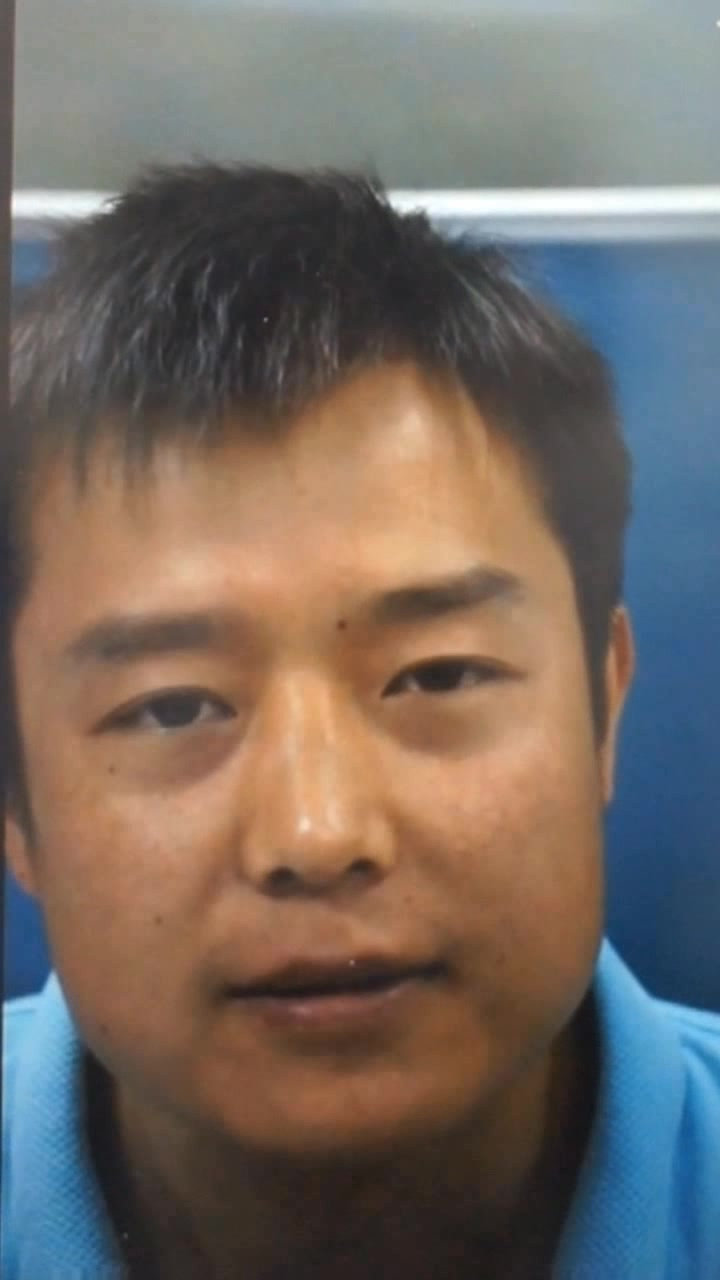
\includegraphics[width=0.2\textwidth]{images_databases/casia/at3-2.jpg}
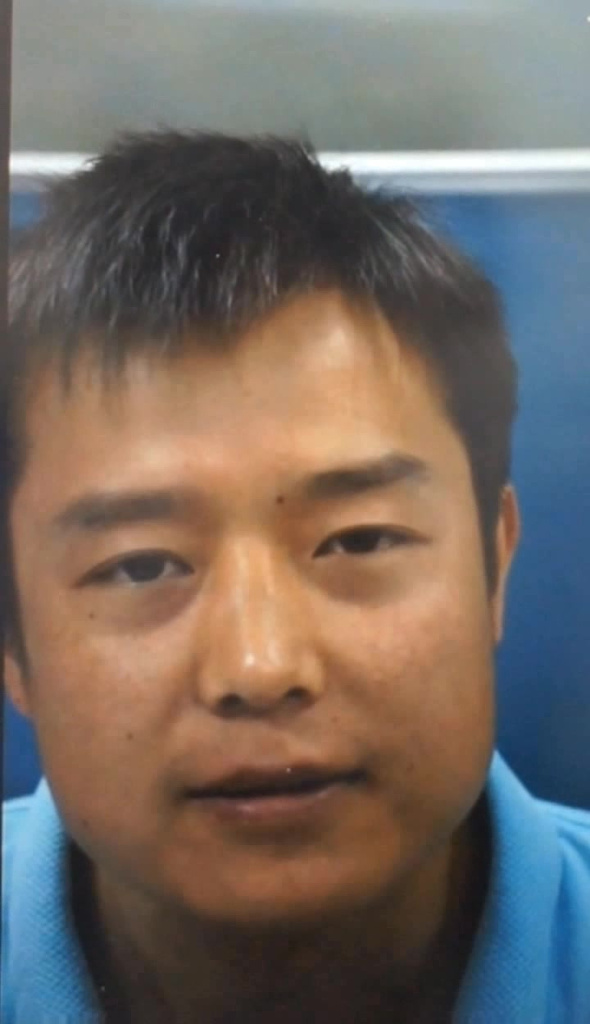
\includegraphics[width=0.2\textwidth]{images_databases/casia/real2.jpg}

\caption{Three attacks and real user from casia database } \label{fig:casia2}
\end{figure}

\begin{figure}[htb]
\centering
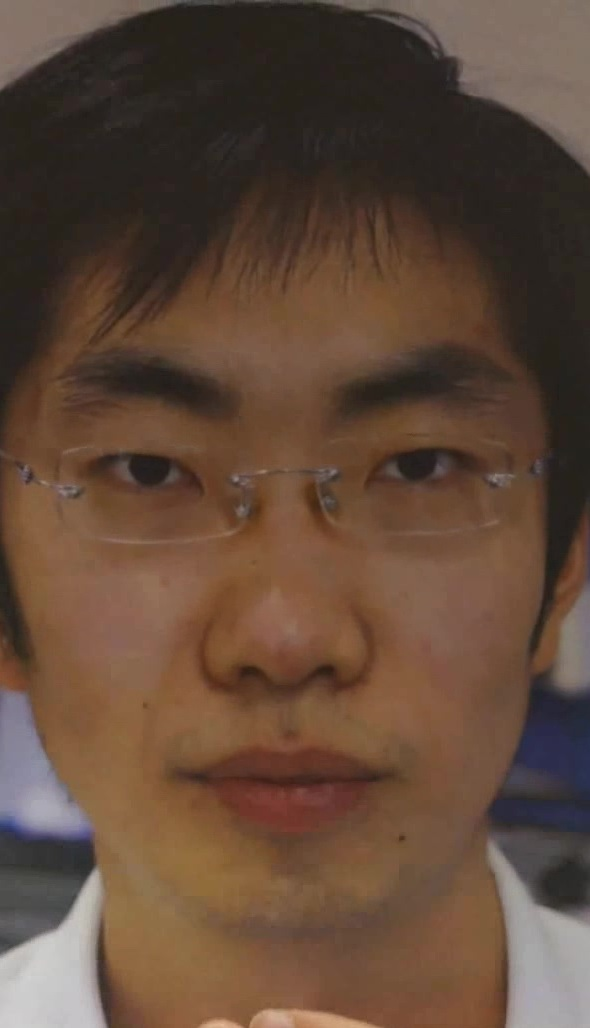
\includegraphics[width=0.2\textwidth]{images_databases/casia/at1-1.jpg}
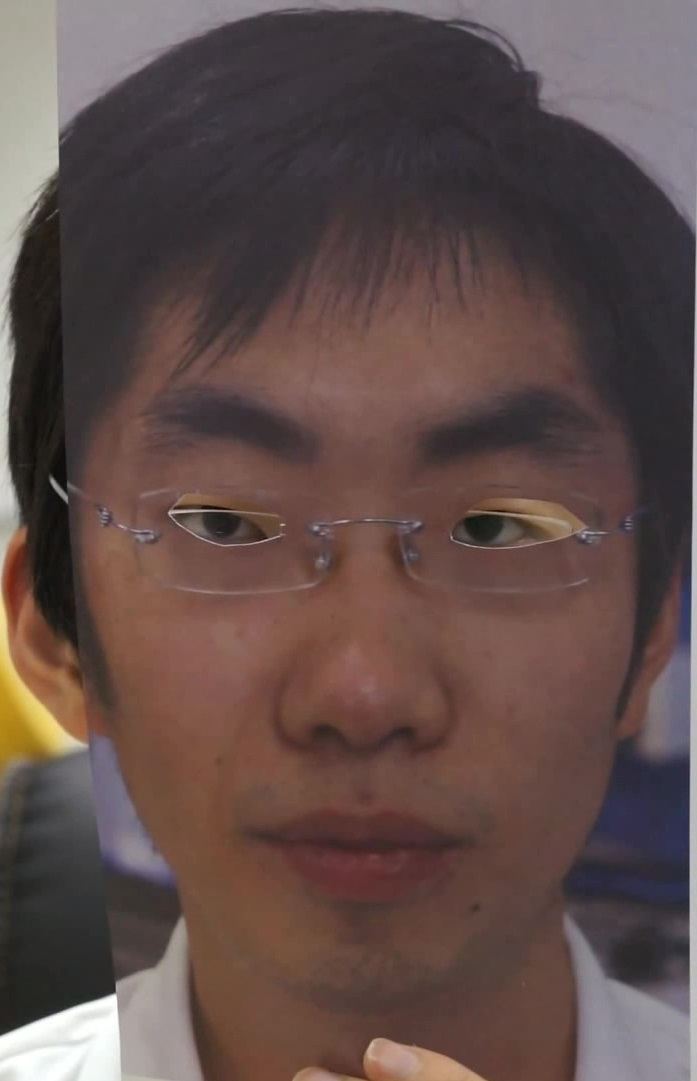
\includegraphics[width=0.2\textwidth]{images_databases/casia/at2-1.jpg}
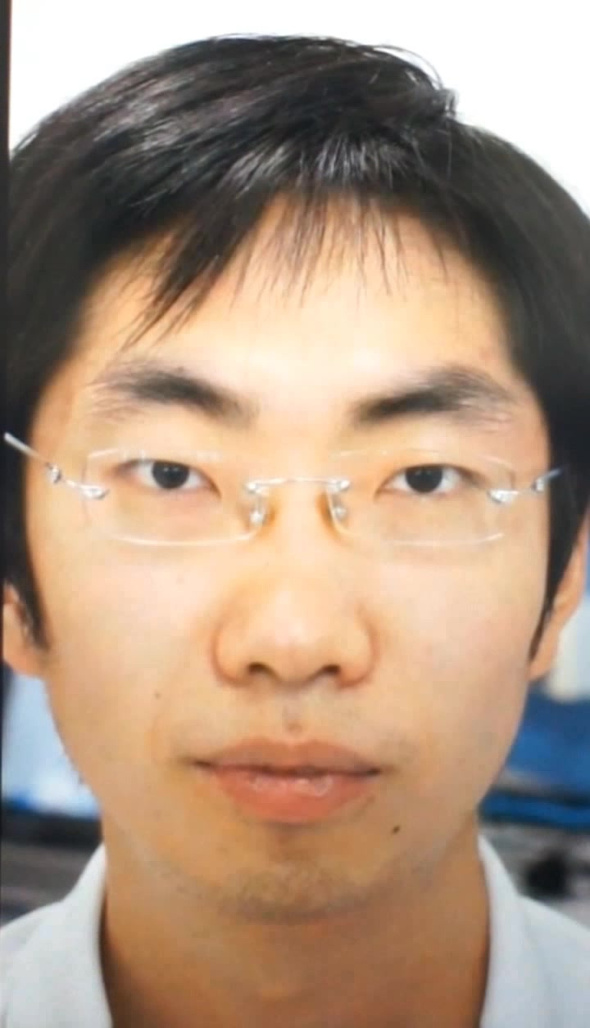
\includegraphics[width=0.2\textwidth]{images_databases/casia/at3-1.jpg}
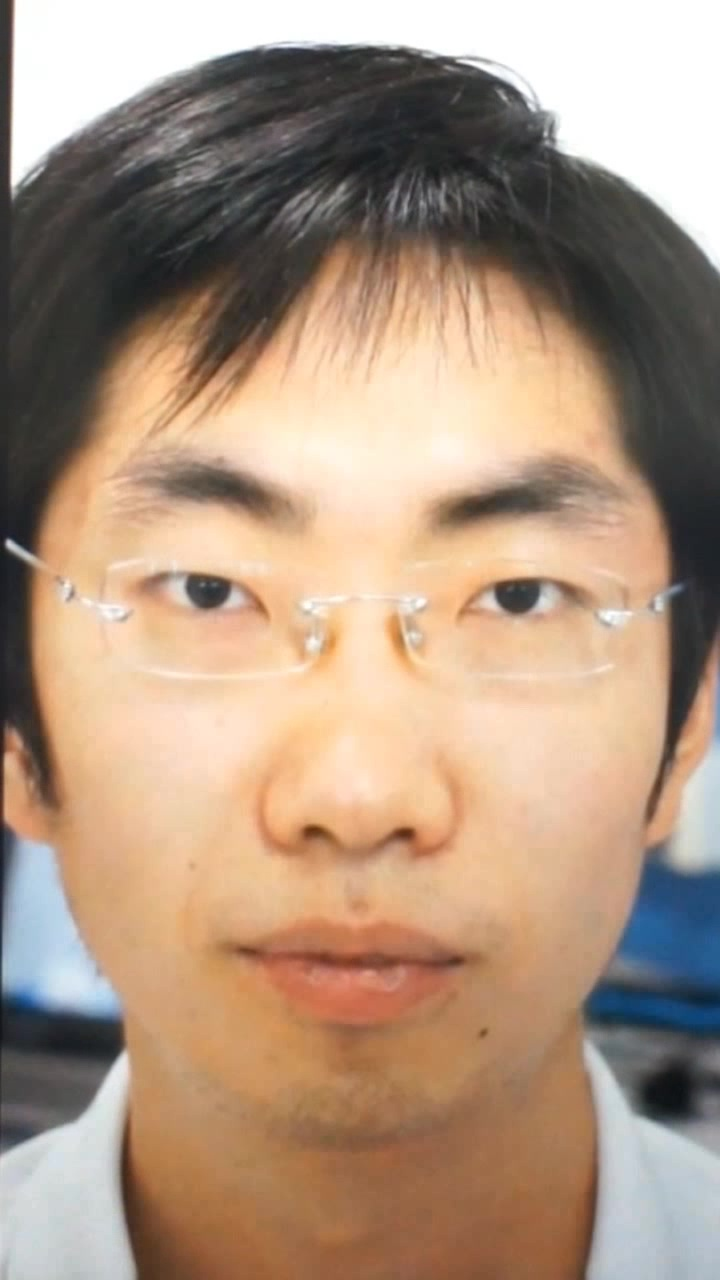
\includegraphics[width=0.2\textwidth]{images_databases/casia/real1.jpg}

\caption{Three attacks and real user from casia database } \label{fig:casia1}
\end{figure}

\subsection{MSU - MFSD database}
The MSU Mobile Face Spoofing Database (MFSD) is a video face anti-spoofing database although for this work just images have been used.\\

The database consist on users and attacks of the same people:\\
\begin{itemize}
\item Genuine users
\item
\end{itemize}

The characteristics of the database are the following ones:\\

\begin{itemize}
\item 35 images per attack or genuine user.
\item Images are RGB.
\item Faces are centered in images.
\item The size of each image are not equal. Approximately images are 300px heigh and 335px width.
\end{itemize}

In figure \ref{fig:mfsd} and figure \ref{fig:mfsd2} It is posible to see the three attacks and the real user.\\

\begin{figure}[htb]
\centering
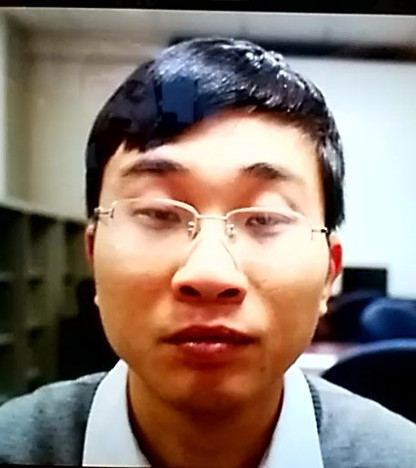
\includegraphics[width=0.2\textwidth]{images_databases/MFSD/at1-1.jpg}
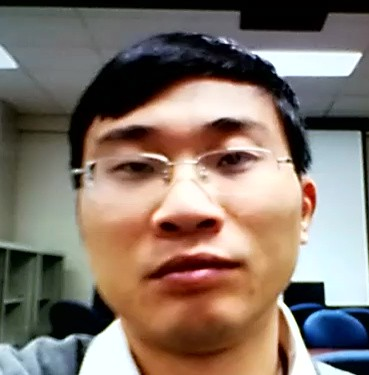
\includegraphics[width=0.2\textwidth]{images_databases/MFSD/at2-1.jpg}
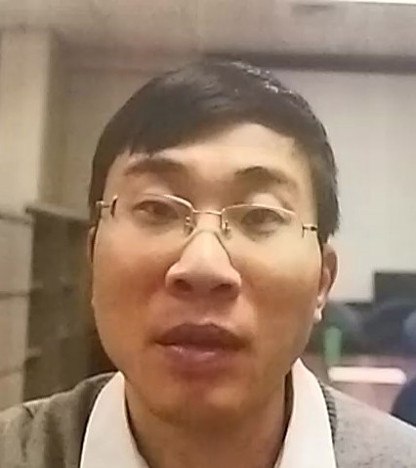
\includegraphics[width=0.2\textwidth]{images_databases/MFSD/at3-1.jpg}
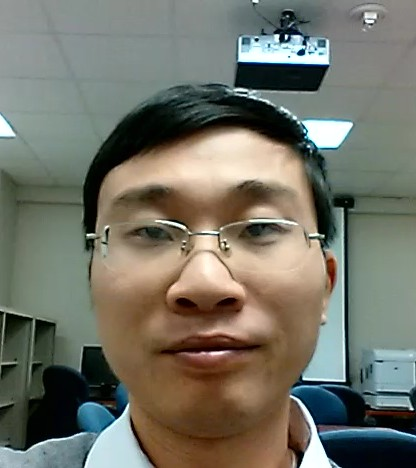
\includegraphics[width=0.2\textwidth]{images_databases/MFSD/1.jpg}
\caption{Three attacks and real user from a user of MFSD database } \label{fig:mfsd}
\end{figure}

\begin{figure}[htb]
\centering
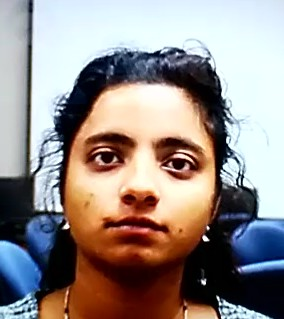
\includegraphics[width=0.2\textwidth]{images_databases/MFSD/at1-2.jpg}
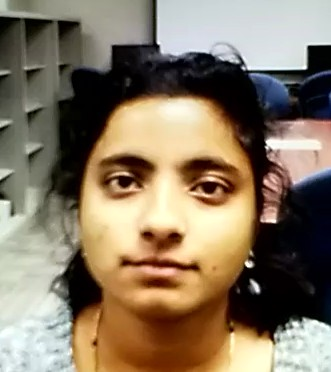
\includegraphics[width=0.2\textwidth]{images_databases/MFSD/at2-2.jpg}
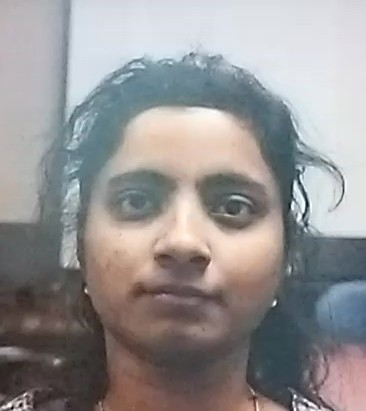
\includegraphics[width=0.2\textwidth]{images_databases/MFSD/at3-2.jpg}
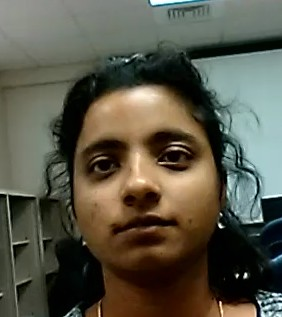
\includegraphics[width=0.2\textwidth]{images_databases/MFSD/2.jpg}
\caption{Three attacks and real user from a user of MFSD database } \label{fig:mfsd2}
\end{figure}
